
\documentclass[letterpaper,hide notes,xcolor={table,svgnames},pdftex,10pt]{beamer}
\def\showexamples{t}


%\usepackage[svgnames]{xcolor}

%% Demo talk
%\documentclass[letterpaper,notes=show]{beamer}

\usecolortheme{crane}
\setbeamertemplate{navigation symbols}{}

\usetheme{MyPittsburgh}
%\usetheme{Frankfurt}

%\usepackage{tipa}

\usepackage{hyperref}
\usepackage{graphicx,xspace}
\usepackage[normalem]{ulem}
\usepackage{multicol}
\usepackage{amsmath,amssymb,amsthm,graphicx,xspace}
\newcommand\SF[1]{$\bigstar$\footnote{SF: #1}}

\usepackage[default]{sourcesanspro}
\usepackage[T1]{fontenc}
\usepackage[scaled]{beramono}
\usepackage{tikzpagenodes}

\newcounter{tmpnumSlide}
\newcounter{tmpnumNote}


% old question code
%\newcommand\question[1]{{$\bigstar$ \small \onlySlide{2}{#1}}}
% \newcommand\nquestion[1]{\ifdefined \presentationonly \textcircled{?} \fi \note{\par{\Large \textbf{?}} #1}}
% \newcommand\nanswer[1]{\note{\par{\Large \textbf{A}} #1}}


 \newcommand\mnote[1]{%
   \addtocounter{tmpnumSlide}{1}
   \ifdefined\showcues {~\tiny\fbox{\arabic{tmpnumSlide}}}\fi
   \note{\setlength{\parskip}{1ex}\addtocounter{tmpnumNote}{1}\textbf{\Large \arabic{tmpnumNote}:} {#1\par}}}

\newcommand\mmnote[1]{\note{\setlength{\parskip}{1ex}#1\par}}

%\newcommand\mnote[2][]{\ifdefined\handoutwithnotes {~\tiny\fbox{#1}}\fi
% \note{\setlength{\parskip}{1ex}\textbf{\Large #1:} #2\par}}

%\newcommand\mnote[2][]{{\tiny\fbox{#1}} \note{\setlength{\parskip}{1ex}\textbf{\Large #1:} #2\par}}

\newcommand\mquestion[2]{{~\color{red}\fbox{?}}\note{\setlength{\parskip}{1ex}\par{\Large \textbf{?}} #1} \note{\setlength{\parskip}{1ex}\par{\Large \textbf{A}} #2\par}\ifdefined \presentationonly \pause \fi}

\newcommand\blackboard[1]{%
\ifdefined   \showblackboard
  {#1}
  \else {\begin{center} \fbox{\colorbox{blue!30}{%
         \begin{minipage}{.95\linewidth}%
           \hspace{\stretch{1}} Some space intentionally left blank; done at the blackboard.%
         \end{minipage}}}\end{center}}%
         \fi%
}



%\newcommand\q{\tikz \node[thick,color=black,shape=circle]{?};}
%\newcommand\q{\ifdefined \presentationonly \textcircled{?} \fi}

\usepackage{listings}
\lstset{basicstyle=\footnotesize\ttfamily,
	breaklines=true,
	aboveskip=15pt,
  	belowskip=15pt,
	frame=lines,
	numbers=left, basicstyle=\scriptsize, numberstyle=\tiny, stepnumber=0, numbersep=2pt
}

\usepackage{siunitx}
\newcommand\sius[1]{\num[group-separator = {,}]{#1}\si{\micro\second}}
\newcommand\sims[1]{\num[group-separator = {,}]{#1}\si{\milli\second}}
\newcommand\sins[1]{\num[group-separator = {,}]{#1}\si{\nano\second}}
\sisetup{group-separator = {,}, group-digits = true}

%% -------------------- tikz --------------------
\usepackage{tikz}
\usetikzlibrary{positioning}
\usetikzlibrary{arrows,backgrounds,automata,decorations.shapes,decorations.pathmorphing,decorations.markings,decorations.text,decorations.pathreplacing}

\tikzstyle{place}=[circle,draw=blue!50,fill=blue!20,thick, inner sep=0pt,minimum size=6mm]
\tikzstyle{transition}=[rectangle,draw=black!50,fill=black!20,thick, inner sep=0pt,minimum size=4mm]

\tikzstyle{block}=[rectangle,draw=black, thick, inner sep=5pt]
\tikzstyle{bullet}=[circle,draw=black, fill=black, thin, inner sep=2pt]

\tikzstyle{pre}=[<-,shorten <=1pt,>=stealth',semithick]
\tikzstyle{post}=[->,shorten >=1pt,>=stealth',semithick]
\tikzstyle{bi}=[<->,shorten >=1pt,shorten <=1pt, >=stealth',semithick]

\tikzstyle{mut}=[-,>=stealth',semithick]

\tikzstyle{treereset}=[dashed,->, shorten >=1pt,>=stealth',thin]

\usepackage{ifmtarg}
\usepackage{xifthen}
\makeatletter
% new counter to now which frame it is within the sequence
\newcounter{multiframecounter}
% initialize buffer for previously used frame title
\gdef\lastframetitle{\textit{undefined}}
% new environment for a multi-frame
\newenvironment{multiframe}[1][]{%
\ifthenelse{\isempty{#1}}{%
% if no frame title was set via optional parameter,
% only increase sequence counter by 1
\addtocounter{multiframecounter}{1}%
}{%
% new frame title has been provided, thus
% reset sequence counter to 1 and buffer frame title for later use
\setcounter{multiframecounter}{1}%
\gdef\lastframetitle{#1}%
}%
% start conventional frame environment and
% automatically set frame title followed by sequence counter
\begin{frame}%
\frametitle{\lastframetitle~{\normalfont(\arabic{multiframecounter})}}%
}{%
\end{frame}%
}
\makeatother

\makeatletter
\newdimen\tu@tmpa%
\newdimen\ydiffl%
\newdimen\xdiffl%
\newcommand\ydiff[2]{%
    \coordinate (tmpnamea) at (#1);%
    \coordinate (tmpnameb) at (#2);%
    \pgfextracty{\tu@tmpa}{\pgfpointanchor{tmpnamea}{center}}%
    \pgfextracty{\ydiffl}{\pgfpointanchor{tmpnameb}{center}}%
    \advance\ydiffl by -\tu@tmpa%
}
\newcommand\xdiff[2]{%
    \coordinate (tmpnamea) at (#1);%
    \coordinate (tmpnameb) at (#2);%
    \pgfextractx{\tu@tmpa}{\pgfpointanchor{tmpnamea}{center}}%
    \pgfextractx{\xdiffl}{\pgfpointanchor{tmpnameb}{center}}%
    \advance\xdiffl by -\tu@tmpa%
}
\makeatother
\newcommand{\copyrightbox}[3][r]{%
\begin{tikzpicture}%
\node[inner sep=0pt,minimum size=2em](ciimage){#2};
\usefont{OT1}{phv}{n}{n}\fontsize{4}{4}\selectfont
\ydiff{ciimage.south}{ciimage.north}
\xdiff{ciimage.west}{ciimage.east}
\ifthenelse{\equal{#1}{r}}{%
\node[inner sep=0pt,right=1ex of ciimage.south east,anchor=north west,rotate=90]%
{\raggedleft\color{black!50}\parbox{\the\ydiffl}{\raggedright{}#3}};%
}{%
\ifthenelse{\equal{#1}{l}}{%
\node[inner sep=0pt,right=1ex of ciimage.south west,anchor=south west,rotate=90]%
{\raggedleft\color{black!50}\parbox{\the\ydiffl}{\raggedright{}#3}};%
}{%
\node[inner sep=0pt,below=1ex of ciimage.south west,anchor=north west]%
{\raggedleft\color{black!50}\parbox{\the\xdiffl}{\raggedright{}#3}};%
}
}
\end{tikzpicture}
}


%% --------------------

%\usepackage[excludeor]{everyhook}
%\PushPreHook{par}{\setbox0=\lastbox\llap{MUH}}\box0}

%\vspace*{\stretch{1}

%\setbox0=\lastbox \llap{\textbullet\enskip}\box0}

\setlength{\parskip}{\fill}

\newcommand\noskips{\setlength{\parskip}{1ex}}
\newcommand\doskips{\setlength{\parskip}{\fill}}

\newcommand\xx{\par\vspace*{\stretch{1}}\par}
\newcommand\xxs{\par\vspace*{2ex}\par}
\newcommand\tuple[1]{\langle #1 \rangle}
\newcommand\code[1]{{\sf \footnotesize #1}}
\newcommand\ex[1]{\uline{Example:} \ifdefined \presentationonly \pause \fi
  \ifdefined\showexamples#1\xspace\else{\uline{\hspace*{2cm}}}\fi}

\newcommand\ceil[1]{\lceil #1 \rceil}


\AtBeginSection[]
{
   \begin{frame}
       \frametitle{Outline}
       \tableofcontents[currentsection]
   \end{frame}
}



\pgfdeclarelayer{edgelayer}
\pgfdeclarelayer{nodelayer}
\pgfsetlayers{edgelayer,nodelayer,main}

\tikzstyle{none}=[inner sep=0pt]
\tikzstyle{rn}=[circle,fill=Red,draw=Black,line width=0.8 pt]
\tikzstyle{gn}=[circle,fill=Lime,draw=Black,line width=0.8 pt]
\tikzstyle{yn}=[circle,fill=Yellow,draw=Black,line width=0.8 pt]
\tikzstyle{empty}=[circle,fill=White,draw=Black]
\tikzstyle{bw} = [rectangle, draw, fill=blue!20, 
    text width=4em, text centered, rounded corners, minimum height=2em]
    
    \newcommand{\CcNote}[1]{% longname
	This work is licensed under the \textit{Creative Commons #1 3.0 License}.%
}
\newcommand{\CcImageBy}[1]{%
	\includegraphics[scale=#1]{creative_commons/cc_by_30.pdf}%
}
\newcommand{\CcImageSa}[1]{%
	\includegraphics[scale=#1]{creative_commons/cc_sa_30.pdf}%
}
\newcommand{\CcImageNc}[1]{%
	\includegraphics[scale=#1]{creative_commons/cc_nc_30.pdf}%
}
\newcommand{\CcGroupBySa}[2]{% zoom, gap
	\CcImageBy{#1}\hspace*{#2}\CcImageNc{#1}\hspace*{#2}\CcImageSa{#1}%
}
\newcommand{\CcLongnameByNcSa}{Attribution-NonCommercial-ShareAlike}

\newenvironment{changemargin}[1]{% 
  \begin{list}{}{% 
    \setlength{\topsep}{0pt}% 
    \setlength{\leftmargin}{#1}% 
    \setlength{\rightmargin}{1em}
    \setlength{\listparindent}{\parindent}% 
    \setlength{\itemindent}{\parindent}% 
    \setlength{\parsep}{\parskip}% 
  }% 
  \item[]}{\end{list}} 




\title{Lecture 24 --- Profiling }

\author{Patrick Lam \\ \small \texttt{patrick.lam@uwaterloo.ca}}
\institute{Department of Electrical and Computer Engineering \\
  University of Waterloo}
\date{\today}


\begin{document}

\begin{frame}
  \titlepage

 \end{frame}


\begin{frame}
\frametitle{Remember the Initial Quiz}


Think back: what operations are fast and what operations are not?

Takeaway: our intuition  is often wrong. 

Not just at a macro level, \\
but at a micro level. 

You may be able to narrow down that this computation of $x$ is slow, \\
but if you examine it carefully\ldots what parts of it are slow?


\end{frame}



\begin{frame}
\frametitle{Premature Optimization}

\vspace*{.5cm}

\begin{quote}
\textit{Programmers waste enormous amounts of time thinking about, or worrying about, the speed of noncritical parts of their programs, and these attempts at efficiency actually have a strong negative impact when debugging and maintenance are considered. We should forget about small efficiencies, say about 97\% of the time: premature optimization is the root of all evil. Yet we should not pass up our opportunities in that critical 3\%.}
\end{quote}
	\hfill -- Donald Knuth


\end{frame}



\begin{frame}
\frametitle{That Saying You Were Expecting}


\begin{changemargin}{1.5cm}
Feeling lucky? \\
Maybe you optimized a slow part. 

\begin{center}
	
\includegraphics[width=0.4\textwidth]{images/feellucky.jpg}
\end{center}

To make your programs or systems fast, \\
you need to find out what is currently slow and improve it (duh!). 

Up until now, it's mostly been about \\
\qquad ``let's speed this up''.\\
We haven't taken much time to decide what we should speed up.
\end{changemargin}

\end{frame}



\begin{frame}
\frametitle{Basic Overview}


\begin{changemargin}{1.5cm}
General idea:\\
\qquad collect data on what parts of the code\\
\qquad are taking up most of the time.

\begin{itemize}
\item What functions get called?
\item How long do functions take?
\item What's using memory?
\end{itemize}
\end{changemargin}

\end{frame}



\begin{frame}
\frametitle{\texttt{printf}}


\begin{changemargin}{1.5cm}
There is always the ``informal'' way: ``debug'' by print statements.

On entry to \texttt{foo}, log ``entering function foo'', plus timestamp.

On exit, log ``exiting foo'', also with timestamp.
\end{changemargin}

\begin{center}
	
\includegraphics[width=0.5\textwidth]{images/stringerbell.jpg}
\end{center}

\end{frame}



\begin{frame}
\frametitle{Console Profiling}


\begin{changemargin}{1cm}
Kind of works, and [JZ] has used it... But this approach is not necessarily good.  

This is ``invasive'' profiling---change the source code of the program to add instrumentation (log statements). 

Plus we have to do a lot of manual accounting.

Doesn't really scale.
\end{changemargin}

\end{frame}



\begin{frame}
\frametitle{Wizardry!}


\begin{changemargin}{2cm}
Like debugging: if you get to be a wizard you can maybe do it by code inspection.

\begin{center}
	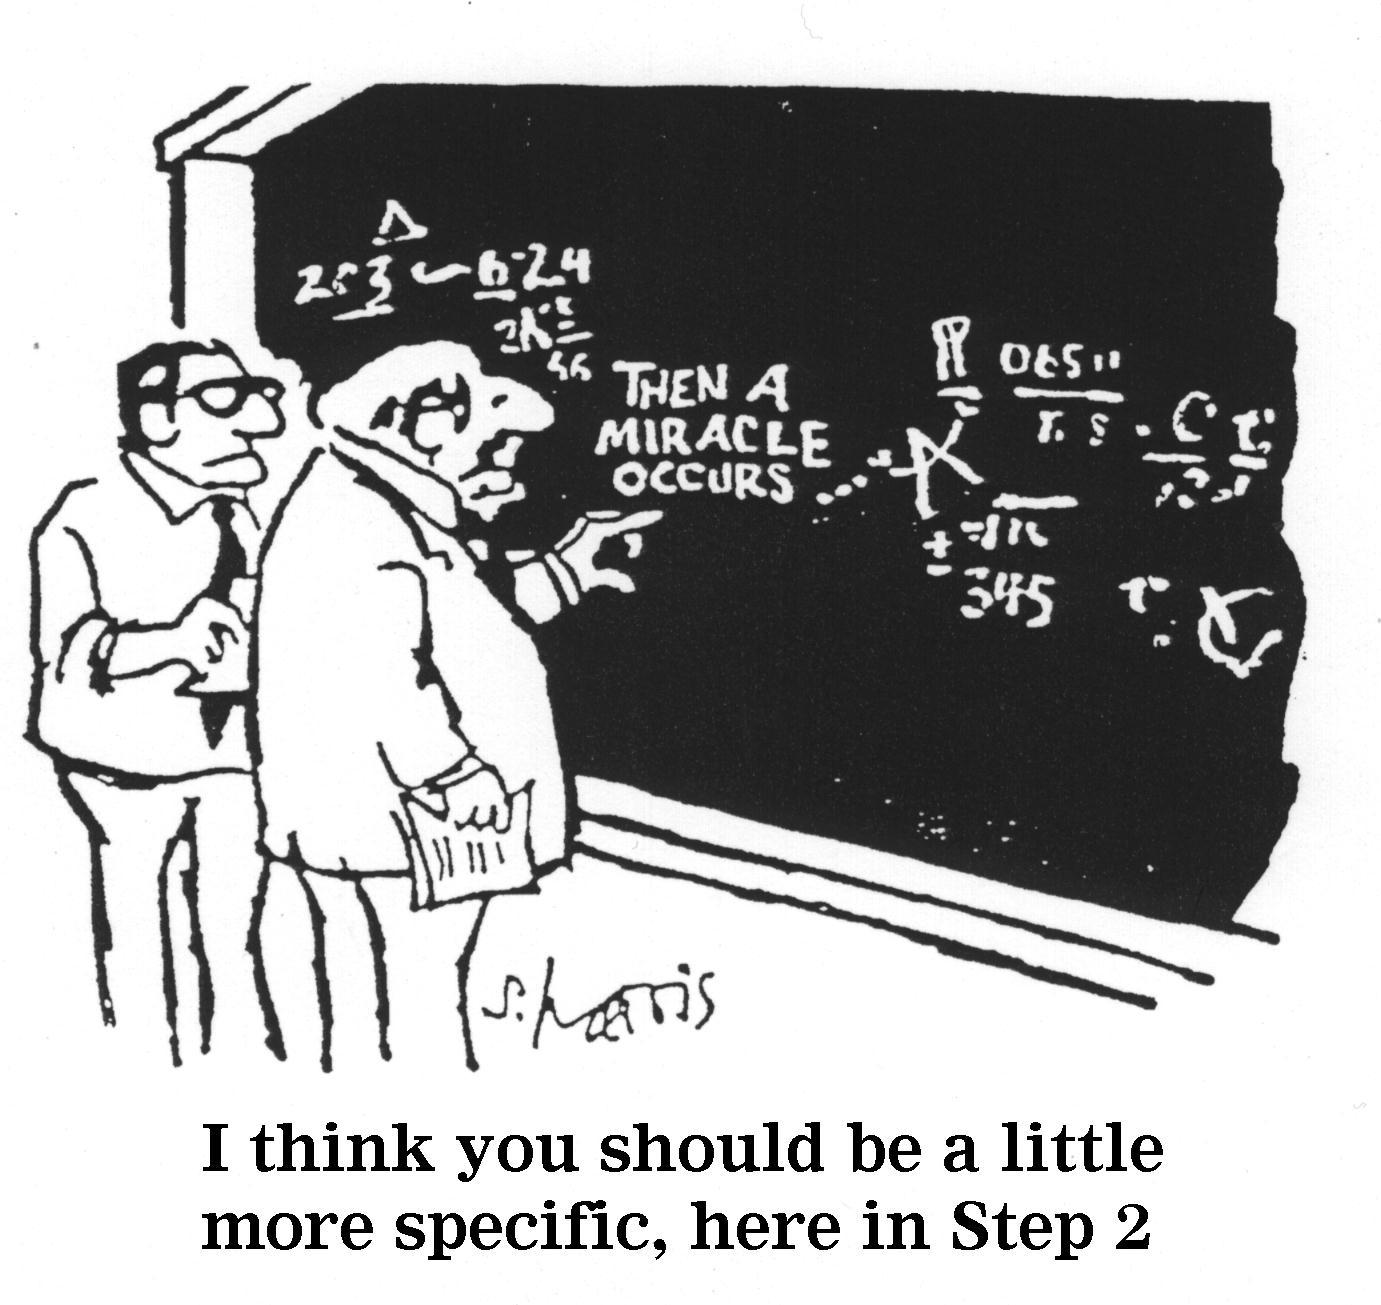
\includegraphics[width=0.4\textwidth]{images/miracle.jpeg}
\end{center}

But speculative execution inside your head is harder for perf than debugging.

So: we want to use tools \\ 
and do this in a methodical way.
\end{changemargin}

\end{frame}


%%%%%%%%%%%%%%%%%%%%%%%%%%%%%%%%%%%%%%%%%%%%%%%%%%%%%%%%%%%%%%%%%%%%%%%%%%%%%%%%
\begin{frame}
  \frametitle{Introduction to Profiling}



\begin{changemargin}{1.5cm}
    So far we've been looking at small problems.\\[1em]
    Must {\bf profile} to see what's slow in a
      large program.\\[1em]
    Two main outputs:
      \begin{itemize}
        \item flat;
        \item call-graph.
      \end{itemize}



    Two main data gathering methods:
      \begin{itemize}
        \item statistical;
        \item instrumentation.
      \end{itemize}
   \end{changemargin}
\end{frame}
%%%%%%%%%%%%%%%%%%%%%%%%%%%%%%%%%%%%%%%%%%%%%%%%%%%%%%%%%%%%%%%%%%%%%%%%%%%%%%%%

%%%%%%%%%%%%%%%%%%%%%%%%%%%%%%%%%%%%%%%%%%%%%%%%%%%%%%%%%%%%%%%%%%%%%%%%%%%%%%%%
\begin{frame}
  \frametitle{Profiler Outputs}


\begin{changemargin}{.5cm}
  
  {\bf Flat Profiler:}

  \begin{itemize}
    \item Only computes average time in a particular function.
    \item Does not include other (useful) information (callees).
  \end{itemize}

~\\[1em]

  {\bf Call-graph Profiler:}

  \begin{itemize}
    \item Computes call times.
    \item Reports frequency of function calls.
    \item Gives a call graph: who called what function?
  \end{itemize}
  \end{changemargin}
\end{frame}
%%%%%%%%%%%%%%%%%%%%%%%%%%%%%%%%%%%%%%%%%%%%%%%%%%%%%%%%%%%%%%%%%%%%%%%%%%%%%%%%

%%%%%%%%%%%%%%%%%%%%%%%%%%%%%%%%%%%%%%%%%%%%%%%%%%%%%%%%%%%%%%%%%%%%%%%%%%%%%%%%
\begin{frame}
  \frametitle{Data Gathering Methods}


\begin{changemargin}{1.5cm}
  {\bf Statistical:}

  Mostly, take samples of the system state, that is:
  \begin{itemize}
    \item every 100ms, check the system state.
    \item will cause some slowdown, but not much.
  \end{itemize}
~\\[1em]

  {\bf Instrumentation:}\\
  Add instructions at specified program points:
  \begin{itemize}
    \item can do this at compile time or run time (expensive);
    \item can instrument either manually or automatically;
    \item like conditional breakpoints.
  \end{itemize}
  \end{changemargin}
\end{frame}
%%%%%%%%%%%%%%%%%%%%%%%%%%%%%%%%%%%%%%%%%%%%%%%%%%%%%%%%%%%%%%%%%%%%%%%%%%%%%%%%

%%%%%%%%%%%%%%%%%%%%%%%%%%%%%%%%%%%%%%%%%%%%%%%%%%%%%%%%%%%%%%%%%%%%%%%%%%%%%%%%
\begin{frame}
  \frametitle{Guide to Profiling}

  

\begin{changemargin}{1cm}
  When writing large software projects:\\[1em]

     $\bullet$ First, write clear and concise code. \\
      \qquad Don't do premature optimizations---\\
      \qquad focus on correctness.\\
     $\bullet$ Profile to get a baseline of your performance:\\[0em]
      \begin{itemize}
        \item allows you to easily track any performance changes;
        \item allows you to re-design your program before it's too late.
      \end{itemize}
  Focus your optimization efforts on the code that matters.
  \end{changemargin}
\end{frame}
%%%%%%%%%%%%%%%%%%%%%%%%%%%%%%%%%%%%%%%%%%%%%%%%%%%%%%%%%%%%%%%%%%%%%%%%%%%%%%%%

%%%%%%%%%%%%%%%%%%%%%%%%%%%%%%%%%%%%%%%%%%%%%%%%%%%%%%%%%%%%%%%%%%%%%%%%%%%%%%%%
\begin{frame}
  \frametitle{Things to Look For}


\begin{changemargin}{1.5cm}
  
    Good signs:\\[0em]

    \begin{itemize}
      \item Time is spent in the right part of the system.
      \item Most time should not be spent handling errors;\\
 in non-critical code; or in exceptional cases.
      \item Time is not unnecessarily spent in OS.
    \end{itemize}
    \end{changemargin}
    
    \begin{center}
	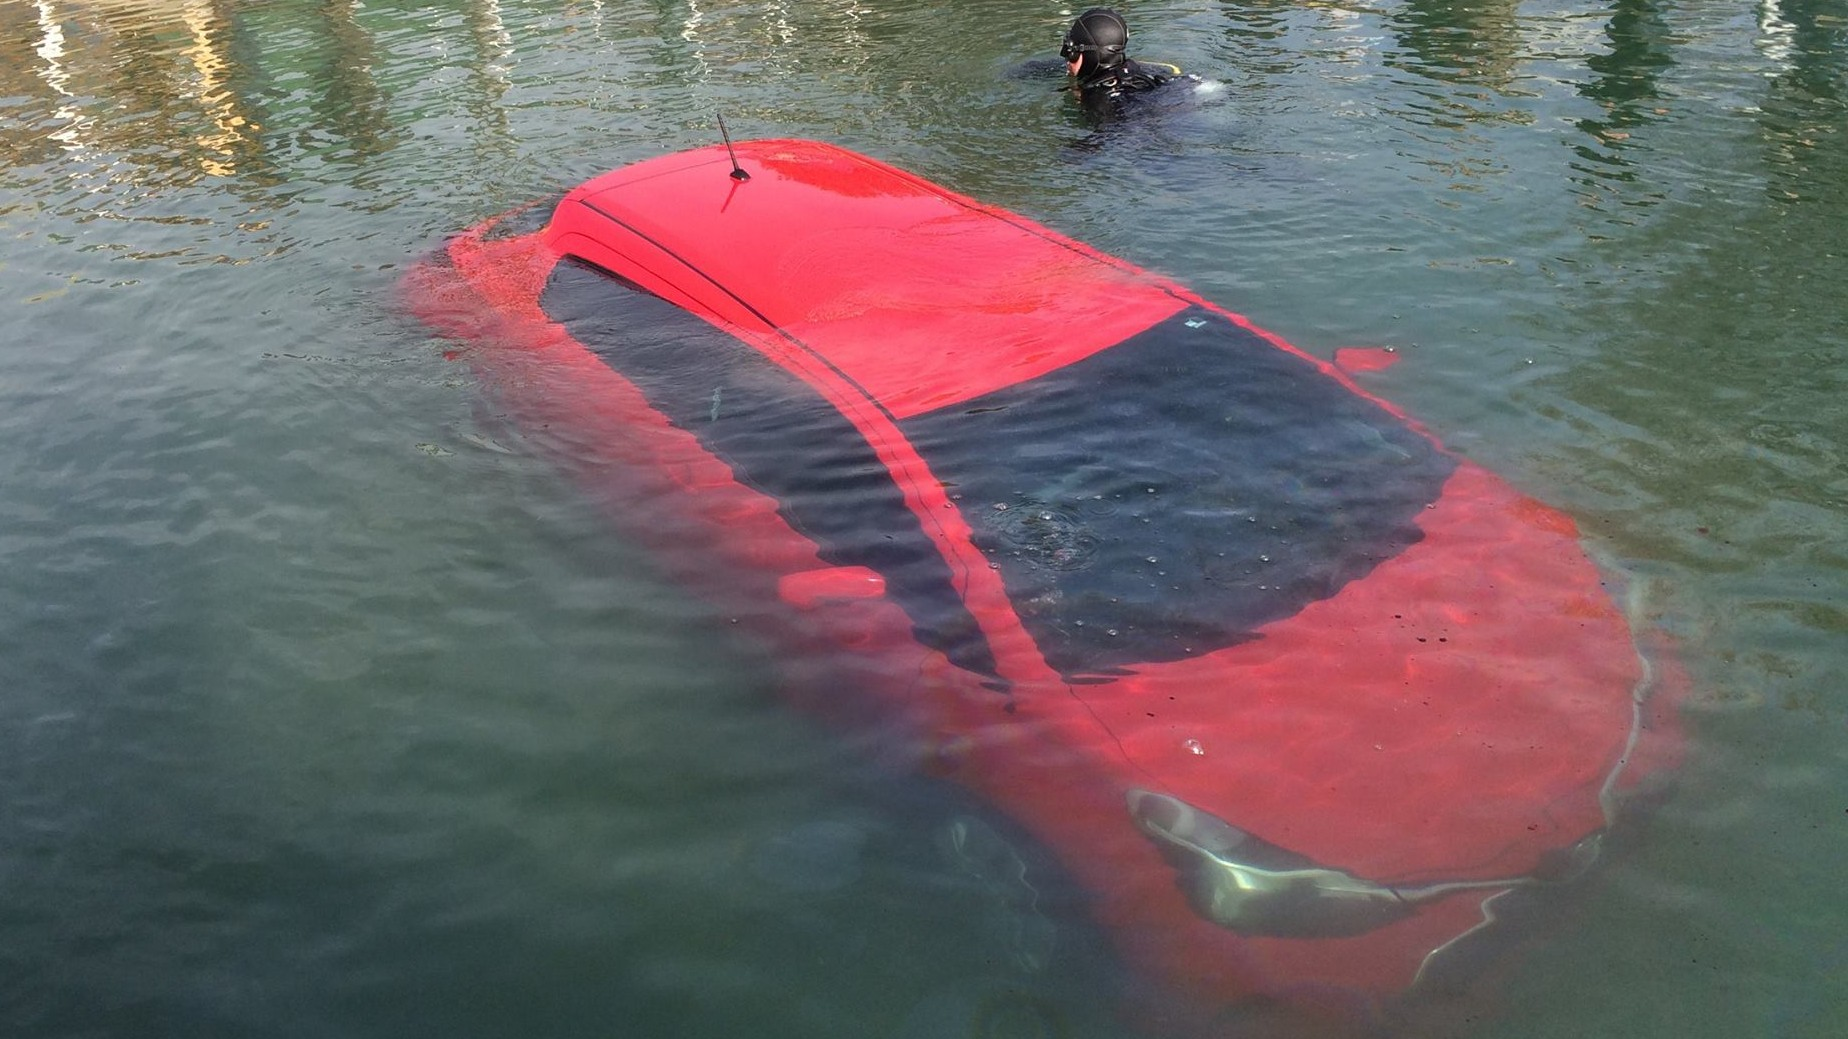
\includegraphics[width=0.5\textwidth]{images/tobermory.jpg}\\
	\hfill Kitchener driver follows GPS directions right into Lake Huron...
 	\end{center}
    
\end{frame}
%%%%%%%%%%%%%%%%%%%%%%%%%%%%%%%%%%%%%%%%%%%%%%%%%%%%%%%%%%%%%%%%%%%%%%%%%%%%%%%%

%%%%%%%%%%%%%%%%%%%%%%%%%%%%%%%%%%%%%%%%%%%%%%%%%%%%%%%%%%%%%%%%%%%%%%%%%%%%%%%%
\begin{frame}
  \frametitle{{\tt gprof} introduction}

  

\begin{changemargin}{1.5cm}
\vspace*{-3em}
    Statistical profiler, plus some instrumentation for calls.\\[1em]
    Runs completely in user-space.\\[1em]
    Only requires a compiler.
    \end{changemargin}
\end{frame}
%%%%%%%%%%%%%%%%%%%%%%%%%%%%%%%%%%%%%%%%%%%%%%%%%%%%%%%%%%%%%%%%%%%%%%%%%%%%%%%%

%%%%%%%%%%%%%%%%%%%%%%%%%%%%%%%%%%%%%%%%%%%%%%%%%%%%%%%%%%%%%%%%%%%%%%%%%%%%%%%%
\begin{frame}
  \frametitle{{\tt gprof} usage}

  

\begin{changemargin}{1.5cm}
\vspace*{-3em}
    Use the {\tt -pg} flag with {\tt clang}.\\[1em]
    Run your program as you normally would.
      \begin{itemize}
        \item Your program will now create a {\tt gmon.out} file.
      \end{itemize}

    Use gprof to interpret the results:\\
 \qquad {\tt gprof <executable>}.
    \end{changemargin}
\end{frame}
%%%%%%%%%%%%%%%%%%%%%%%%%%%%%%%%%%%%%%%%%%%%%%%%%%%%%%%%%%%%%%%%%%%%%%%%%%%%%%%%

%%%%%%%%%%%%%%%%%%%%%%%%%%%%%%%%%%%%%%%%%%%%%%%%%%%%%%%%%%%%%%%%%%%%%%%%%%%%%%%%
\begin{frame}[fragile]
  \frametitle{{\tt gprof} example}

  

\begin{changemargin}{1.5cm}
    A program with 100 million calls to two math functions.

  \begin{lstlisting}
int main() {
    int i,x1=10,y1=3,r1=0;
    float x2=10,y2=3,r2=0;

    for(i=0;i<100000000;i++) {
        r1 += int_math(x1,y1);
        r2 += float_math(y2,y2);
    }
}
  \end{lstlisting}

  \begin{itemize}
    \item Looking at the code, we have no idea what takes longer.
    \item Probably would guess floating point math taking longer.
    \item (Overall, silly example.)
  \end{itemize}
  \end{changemargin}
\end{frame}
%%%%%%%%%%%%%%%%%%%%%%%%%%%%%%%%%%%%%%%%%%%%%%%%%%%%%%%%%%%%%%%%%%%%%%%%%%%%%%%%

%%%%%%%%%%%%%%%%%%%%%%%%%%%%%%%%%%%%%%%%%%%%%%%%%%%%%%%%%%%%%%%%%%%%%%%%%%%%%%%%
\begin{frame}[fragile]
  \frametitle{Example (Integer Math)}

  

\begin{changemargin}{1.5cm}
  \begin{lstlisting}
int int_math(int x, int y){
    int r1;
    r1=int_power(x,y);
    r1=int_math_helper(x,y);
    return r1;
}

int int_math_helper(int x, int y){
    int r1;
    r1=x/y*int_power(y,x)/int_power(x,y);
    return r1;
}

int int_power(int x, int y){
    int i, r;
    r=x;
    for(i=1;i<y;i++){
        r=r*x;
    }
    return r;
}
  \end{lstlisting}
  \end{changemargin}
\end{frame}
%%%%%%%%%%%%%%%%%%%%%%%%%%%%%%%%%%%%%%%%%%%%%%%%%%%%%%%%%%%%%%%%%%%%%%%%%%%%%%%%


%%%%%%%%%%%%%%%%%%%%%%%%%%%%%%%%%%%%%%%%%%%%%%%%%%%%%%%%%%%%%%%%%%%%%%%%%%%%%%%%
\begin{frame}[fragile]
  \frametitle{Example (Float Math)}


\begin{changemargin}{1.5cm}
  
  \begin{lstlisting}
float float_math(float x, float y) {
    float r1;
    r1=float_power(x,y);
    r1=float_math_helper(x,y);
    return r1;
}

float float_math_helper(float x, float y) {
    float r1;
    r1=x/y*float_power(y,x)/float_power(x,y);
    return r1;
}

float float_power(float x, float y){
    float i, r;
    r=x;
    for(i=1;i<y;i++) {
        r=r*x;
    }
    return r;
}
  \end{lstlisting}
  \end{changemargin}

\end{frame}
%%%%%%%%%%%%%%%%%%%%%%%%%%%%%%%%%%%%%%%%%%%%%%%%%%%%%%%%%%%%%%%%%%%%%%%%%%%%%%%%

%%%%%%%%%%%%%%%%%%%%%%%%%%%%%%%%%%%%%%%%%%%%%%%%%%%%%%%%%%%%%%%%%%%%%%%%%%%%%%%%
\begin{frame}[fragile]
  \frametitle{Flat Profile}


\begin{changemargin}{1.5cm}

    When we run the program, profile says:

{
  \begin{lstlisting}[basicstyle=\tiny]
Flat profile:

Each sample counts as 0.01 seconds.
  %   cumulative   self              self     total           
 time   seconds   seconds    calls  ns/call  ns/call  name    
 32.58      4.69     4.69 300000000    15.64    15.64  int_power
 30.55      9.09     4.40 300000000    14.66    14.66  float_power
 16.95     11.53     2.44 100000000    24.41    55.68  int_math_helper
 11.43     13.18     1.65 100000000    16.46    45.78  float_math_helper
  4.05     13.76     0.58 100000000     5.84    77.16  int_math
  3.01     14.19     0.43 100000000     4.33    64.78  float_math
  2.10     14.50     0.30                             main
  \end{lstlisting}
}

  \begin{itemize}
    \item One function per line.
    \item {\bf \% time:} the percent of the total execution time in this function.
    \item {\bf self:} seconds in this function.
    \item {\bf cumulative:} sum of this function's time + any above it in table.
  \end{itemize}
  \end{changemargin}
\end{frame}
%%%%%%%%%%%%%%%%%%%%%%%%%%%%%%%%%%%%%%%%%%%%%%%%%%%%%%%%%%%%%%%%%%%%%%%%%%%%%%%%

%%%%%%%%%%%%%%%%%%%%%%%%%%%%%%%%%%%%%%%%%%%%%%%%%%%%%%%%%%%%%%%%%%%%%%%%%%%%%%%%
\begin{frame}[fragile]
  \frametitle{Flat Profile}



\begin{changemargin}{1.5cm}
  \begin{lstlisting}[basicstyle=\tiny]
Flat profile:

Each sample counts as 0.01 seconds.
  %   cumulative   self              self     total           
 time   seconds   seconds    calls  ns/call  ns/call  name    
 32.58      4.69     4.69 300000000    15.64    15.64  int_power
 30.55      9.09     4.40 300000000    14.66    14.66  float_power
 16.95     11.53     2.44 100000000    24.41    55.68  int_math_helper
 11.43     13.18     1.65 100000000    16.46    45.78  float_math_helper
  4.05     13.76     0.58 100000000     5.84    77.16  int_math
  3.01     14.19     0.43 100000000     4.33    64.78  float_math
  2.10     14.50     0.30                             main
  \end{lstlisting}


  \begin{itemize}
    \item {\bf calls:} number of times this function was called
    \item {\bf self ns/call:} just self nanoseconds / calls
    \item {\bf total ns/call:} average time for function execution, including
      any other calls the function makes
  \end{itemize}
  \end{changemargin}
\end{frame}
%%%%%%%%%%%%%%%%%%%%%%%%%%%%%%%%%%%%%%%%%%%%%%%%%%%%%%%%%%%%%%%%%%%%%%%%%%%%%%%%

%%%%%%%%%%%%%%%%%%%%%%%%%%%%%%%%%%%%%%%%%%%%%%%%%%%%%%%%%%%%%%%%%%%%%%%%%%%%%%%%
\begin{frame}[fragile]
  \frametitle{Call Graph Example (1)}


\begin{changemargin}{1.5cm}
  
    After the flat profile gives you a feel for which functions are costly, 
      can get a better story from the call graph.
  \vfill
  \begin{lstlisting}[basicstyle=\tiny]
index % time    self  children    called     name
                                                 <spontaneous>
[1]    100.0    0.30   14.19                 main [1]
                0.58    7.13 100000000/100000000     int_math [2]
                0.43    6.04 100000000/100000000     float_math [3]
-----------------------------------------------
                0.58    7.13 100000000/100000000     main [1]
[2]     53.2    0.58    7.13 100000000         int_math [2]
                2.44    3.13 100000000/100000000     int_math_helper [4]
                1.56    0.00 100000000/300000000     int_power [5]
-----------------------------------------------
                0.43    6.04 100000000/100000000     main [1]
[3]     44.7    0.43    6.04 100000000         float_math [3]
                1.65    2.93 100000000/100000000     float_math_helper [6]
                1.47    0.00 100000000/300000000     float_power [7]
  \end{lstlisting}
  \end{changemargin}
\end{frame}
%%%%%%%%%%%%%%%%%%%%%%%%%%%%%%%%%%%%%%%%%%%%%%%%%%%%%%%%%%%%%%%%%%%%%%%%%%%%%%%%

%%%%%%%%%%%%%%%%%%%%%%%%%%%%%%%%%%%%%%%%%%%%%%%%%%%%%%%%%%%%%%%%%%%%%%%%%%%%%%%%
\begin{frame}[fragile]
  \frametitle{Reading the Call Graph}


\begin{changemargin}{1.5cm}
  
    The line with the index is the current function being looked at {\bf (primary line)}.\\
\begin{itemize}
    \item Lines above are functions which called this function.
    \item Lines below are functions which were called by this function
      (children).
  \end{itemize}
~\\
  {\bf Primary Line}

  \begin{itemize}  
    \item {\bf time:} total percentage of time spent in this function and its
      children
    \item {\bf self:} same as in flat profile
    \item {\bf children:} time spent in all calls made by the function
      \begin{itemize}
        \item should be equal to self + children of all functions below
      \end{itemize}
  \end{itemize}
  \end{changemargin}
\end{frame}
%%%%%%%%%%%%%%%%%%%%%%%%%%%%%%%%%%%%%%%%%%%%%%%%%%%%%%%%%%%%%%%%%%%%%%%%%%%%%%%%

%%%%%%%%%%%%%%%%%%%%%%%%%%%%%%%%%%%%%%%%%%%%%%%%%%%%%%%%%%%%%%%%%%%%%%%%%%%%%%%%
\begin{frame}[fragile]
  \frametitle{Reading Callers from Call Graph}

  

\begin{changemargin}{1.5cm}
  {\bf Callers (functions above the primary line)}
  \begin{itemize}  
    \item {\bf self:} time spent in primary function, when called from current
      function.
    \item {\bf children:} time spent in primary function's children, when
      called from current function.
    \item {\bf called:} number of times primary function was called from current
      function / number of nonrecursive calls to primary function.
  \end{itemize}
  \end{changemargin}
\end{frame}
%%%%%%%%%%%%%%%%%%%%%%%%%%%%%%%%%%%%%%%%%%%%%%%%%%%%%%%%%%%%%%%%%%%%%%%%%%%%%%%%

%%%%%%%%%%%%%%%%%%%%%%%%%%%%%%%%%%%%%%%%%%%%%%%%%%%%%%%%%%%%%%%%%%%%%%%%%%%%%%%%
\begin{frame}[fragile]
  \frametitle{Reading Callees from Call Graph}


\begin{changemargin}{1.5cm}
  
  {\bf Callees (functions below the primary line)}
  \begin{itemize}  
    \item {\bf self:} time spent in current function when called from primary.
    \item {\bf children:} time spent in current function's children calls when
      called from primary.
      \begin{itemize}
        \item self + children is an estimate of time spent in current function
          when called from primary function.
      \end{itemize}
    \item {\bf called:} number of times current function was called from primary
      function / number of nonrecursive calls to current function.
  \end{itemize}
  \end{changemargin}
\end{frame}
%%%%%%%%%%%%%%%%%%%%%%%%%%%%%%%%%%%%%%%%%%%%%%%%%%%%%%%%%%%%%%%%%%%%%%%%%%%%%%%%

%%%%%%%%%%%%%%%%%%%%%%%%%%%%%%%%%%%%%%%%%%%%%%%%%%%%%%%%%%%%%%%%%%%%%%%%%%%%%%%%
\begin{frame}[fragile]
  \frametitle{Call Graph Example (2)}


\begin{changemargin}{1.5cm}
  
  \begin{lstlisting}[basicstyle=\tiny]
index % time    self  children    called     name

                2.44    3.13 100000000/100000000     int_math [2]
[4]     38.4    2.44    3.13 100000000         int_math_helper [4]
                3.13    0.00 200000000/300000000     int_power [5]
-----------------------------------------------
                1.56    0.00 100000000/300000000     int_math [2]
                3.13    0.00 200000000/300000000     int_math_helper [4]
[5]     32.4    4.69    0.00 300000000         int_power [5]
-----------------------------------------------
                1.65    2.93 100000000/100000000     float_math [3]
[6]     31.6    1.65    2.93 100000000         float_math_helper [6]
                2.93    0.00 200000000/300000000     float_power [7]
-----------------------------------------------
                1.47    0.00 100000000/300000000     float_math [3]
                2.93    0.00 200000000/300000000     float_math_helper [6]
[7]     30.3    4.40    0.00 300000000         float_power [7]
  \end{lstlisting}

  
 We can now see where most of the time comes from, and pinpoint 
      locations that make unexpected calls, etc.\\[1em]
 This example isn't too exciting; could simplify the math.
 \end{changemargin}
\end{frame}
%%%%%%%%%%%%%%%%%%%%%%%%%%%%%%%%%%%%%%%%%%%%%%%%%%%%%%%%%%%%%%%%%%%%%%%%%%%%%%%%

%%%%%%%%%%%%%%%%%%%%%%%%%%%%%%%%%%%%%%%%%%%%%%%%%%%%%%%%%%%%%%%%%%%%%%%%%%%%%%%%
\begin{frame}
  \frametitle{Introduction to gperftools}


\begin{changemargin}{1.5cm}

    Google Performance Tools include:
      
      \begin{itemize}
        \item CPU profiler.
        \item Heap profiler.
        \item Heap checker.
        \item Faster (multithreaded) {\tt malloc}.
      \end{itemize}
~\\[-1em]
     We'll mostly use the CPU profiler:
      \begin{itemize}
        \item purely statistical sampling;
        \item no recompilation; at most linking; and
        \item built-in visual output.
      \end{itemize}
      \end{changemargin}
\end{frame}
%%%%%%%%%%%%%%%%%%%%%%%%%%%%%%%%%%%%%%%%%%%%%%%%%%%%%%%%%%%%%%%%%%%%%%%%%%%%%%%%

%%%%%%%%%%%%%%%%%%%%%%%%%%%%%%%%%%%%%%%%%%%%%%%%%%%%%%%%%%%%%%%%%%%%%%%%%%%%%%%%
\begin{frame}[fragile]
  \frametitle{Google Perf Tools profiler usage}

  

\begin{changemargin}{1.5cm}
    You can use the profiler without any recompilation.
      \begin{itemize}
        \item Not recommended---worse data.
      \end{itemize}

  \begin{lstlisting}
LD_PRELOAD="/usr/lib/libprofiler.so" \
CPUPROFILE=test.prof ./test
  \end{lstlisting}

     The other option is to link to the profiler:
      \begin{itemize}
        \item {\tt -lprofiler}
      \end{itemize}
    Both options read the {\tt CPUPROFILE} environment variable:
      \begin{itemize}
        \item states the location to write the profile data.
      \end{itemize}
      \end{changemargin}
\end{frame}
%%%%%%%%%%%%%%%%%%%%%%%%%%%%%%%%%%%%%%%%%%%%%%%%%%%%%%%%%%%%%%%%%%%%%%%%%%%%%%%%

%%%%%%%%%%%%%%%%%%%%%%%%%%%%%%%%%%%%%%%%%%%%%%%%%%%%%%%%%%%%%%%%%%%%%%%%%%%%%%%%
\begin{frame}[fragile]
  \frametitle{Other Usage}


\begin{changemargin}{1.5cm}
  
     You can use the profiling library directly as well:
      \begin{itemize}
        \item {\tt \#include <gperftools/profiler.h>}
      \end{itemize}
     Bracket code you want profiled with:
      \begin{itemize}
        \item {\tt ProfilerStart()}
        \item {\tt ProfilerStop()}
      \end{itemize}~\\
    
    You can change the sampling frequency with the
      {\tt CPUPROFILE\_FREQUENCY} environment variable.
      \begin{itemize}
        \item {\bf Default value:} 100
      \end{itemize}
      \end{changemargin}
\end{frame}
%%%%%%%%%%%%%%%%%%%%%%%%%%%%%%%%%%%%%%%%%%%%%%%%%%%%%%%%%%%%%%%%%%%%%%%%%%%%%%%%

%%%%%%%%%%%%%%%%%%%%%%%%%%%%%%%%%%%%%%%%%%%%%%%%%%%%%%%%%%%%%%%%%%%%%%%%%%%%%%%%
\begin{frame}[fragile]
  \frametitle{{\tt pprof} Usage}



\begin{changemargin}{1.5cm}
    Like {\tt gprof}, it will analyze profiling results.

  \begin{lstlisting}
% pprof test test.prof
    Enters "interactive" mode
% pprof --text test test.prof
    Outputs one line per procedure
% pprof --gv test test.prof
     Displays annotated call-graph via 'gv'
% pprof --gv --focus=Mutex test test.prof
    Restricts to code paths including a .*Mutex.* entry
% pprof --gv --focus=Mutex --ignore=string test test.prof
    Code paths including Mutex but not string
% pprof --list=getdir test test.prof
    (Per-line) annotated source listing for getdir()
% pprof --disasm=getdir test test.prof
    (Per-PC) annotated disassembly for getdir()
  \end{lstlisting}

    Can also output {\tt dot}, {\tt ps}, {\tt pdf} or {\tt gif} instead of
      {\tt gv}.
      \end{changemargin}

\end{frame}
%%%%%%%%%%%%%%%%%%%%%%%%%%%%%%%%%%%%%%%%%%%%%%%%%%%%%%%%%%%%%%%%%%%%%%%%%%%%%%%%

%%%%%%%%%%%%%%%%%%%%%%%%%%%%%%%%%%%%%%%%%%%%%%%%%%%%%%%%%%%%%%%%%%%%%%%%%%%%%%%%
\begin{frame}[fragile]
  \frametitle{Text Output}


\begin{changemargin}{1.5cm}

    Similar to the flat profile in {\tt gprof}

  \begin{lstlisting}
jon@riker examples master % pprof --text test test.prof 
Using local file test.
Using local file test.prof.
Removing killpg from all stack traces.
Total: 300 samples
      95  31.7%  31.7%      102  34.0% int_power
      58  19.3%  51.0%       58  19.3% float_power
      51  17.0%  68.0%       96  32.0% float_math_helper
      50  16.7%  84.7%      137  45.7% int_math_helper
      18   6.0%  90.7%      131  43.7% float_math
      14   4.7%  95.3%      159  53.0% int_math
      14   4.7% 100.0%      300 100.0% main
       0   0.0% 100.0%      300 100.0% __libc_start_main
       0   0.0% 100.0%      300 100.0% _start
  \end{lstlisting}
  
  \end{changemargin}
\end{frame}
%%%%%%%%%%%%%%%%%%%%%%%%%%%%%%%%%%%%%%%%%%%%%%%%%%%%%%%%%%%%%%%%%%%%%%%%%%%%%%%%

%%%%%%%%%%%%%%%%%%%%%%%%%%%%%%%%%%%%%%%%%%%%%%%%%%%%%%%%%%%%%%%%%%%%%%%%%%%%%%%%
\begin{frame}
  \frametitle{Text Output Explained}


\begin{changemargin}{1.5cm}
  
    Columns, from left to right:\\[1em]

    Number of checks (samples) in this function.\\
    Percentage of checks in this function.
      \begin{itemize}
        \item Same as {\bf time} in {\tt gprof}.\\[1em]
      \end{itemize}
    Percentage of checks in the functions printed so far.
      \begin{itemize}
        \item Equivalent to {\bf cumulative} (but in \%).\\[1em]
      \end{itemize}
    Number of checks in this function and its callees.\\
    Percentage of checks in this function and its callees.\\
    Function name.
    \end{changemargin}
\end{frame}
%%%%%%%%%%%%%%%%%%%%%%%%%%%%%%%%%%%%%%%%%%%%%%%%%%%%%%%%%%%%%%%%%%%%%%%%%%%%%%%%

%%%%%%%%%%%%%%%%%%%%%%%%%%%%%%%%%%%%%%%%%%%%%%%%%%%%%%%%%%%%%%%%%%%%%%%%%%%%%%%%
\begin{frame}
  \frametitle{Graphical Output}

  \begin{center}
    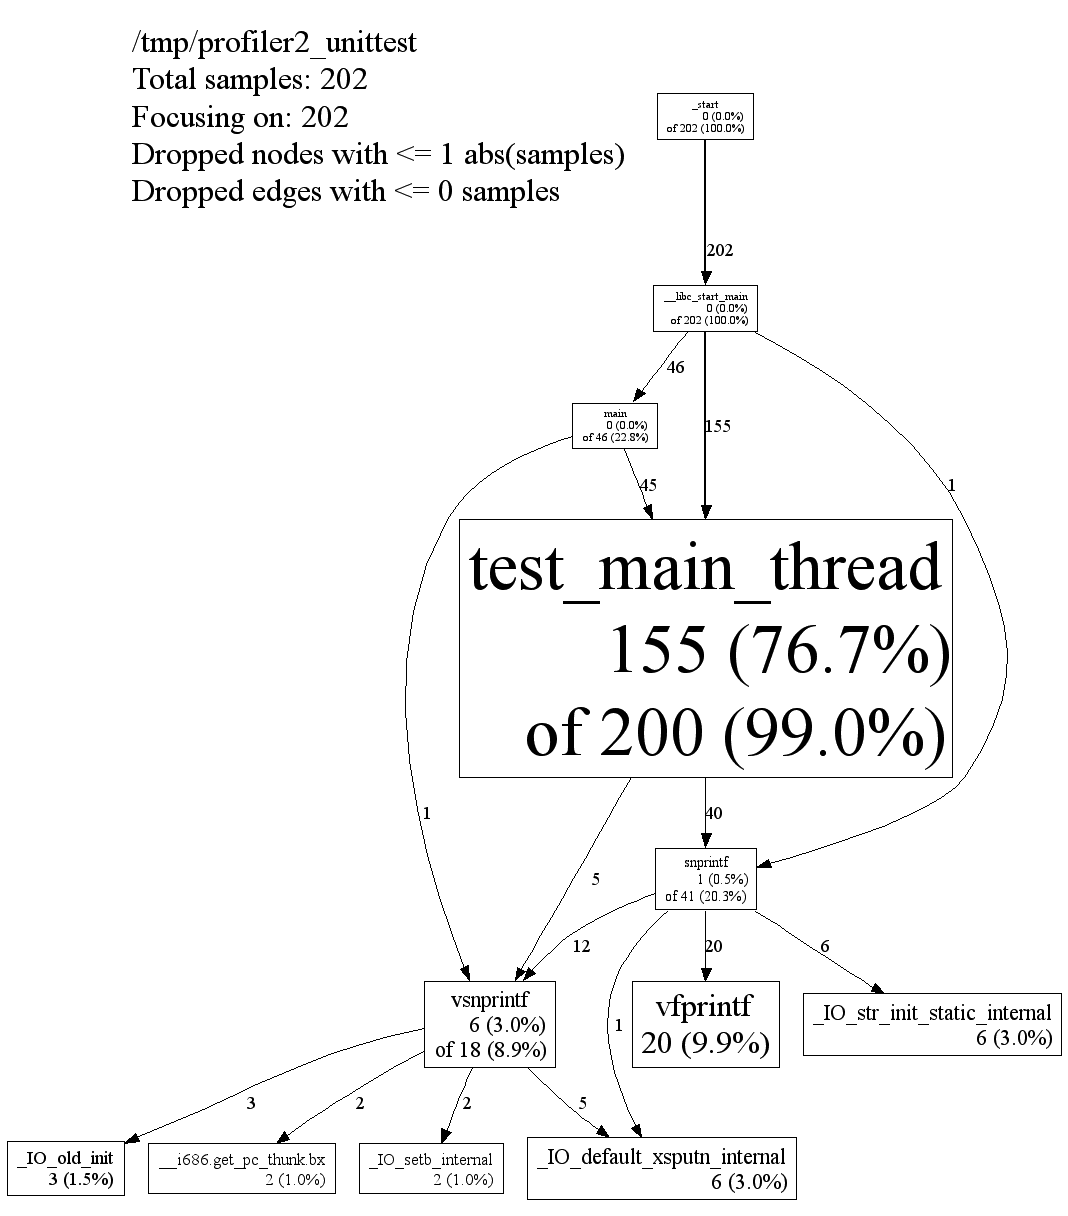
\includegraphics[width=0.5\textwidth]{images/pprof-test-big.png}
  \end{center}
\end{frame}
%%%%%%%%%%%%%%%%%%%%%%%%%%%%%%%%%%%%%%%%%%%%%%%%%%%%%%%%%%%%%%%%%%%%%%%%%%%%%%%%

%%%%%%%%%%%%%%%%%%%%%%%%%%%%%%%%%%%%%%%%%%%%%%%%%%%%%%%%%%%%%%%%%%%%%%%%%%%%%%%%
\begin{frame}
  \frametitle{Graphical Output Explained}


\begin{changemargin}{1.5cm}
  
  Output was too small to read on the slide.

  \begin{itemize}
    \item Shows the same numbers as the text output.
    \item Directed edges denote function calls.
    \item Note: number of samples in callees = \\
      \qquad number in ``this function + callees'' - \\
      \qquad number in ``this function''.\\
    \item {\bf Example:}\\
{{\tt float\_math\_helper}, 51 (local) of 96 (cumulative)} \\
      96 - 51 = 45 (callees)
      \begin{itemize}
        \item callee {\tt int\_power} = 7 (bogus)
        \item callee {\tt float\_power} = 38
        \item callees total = 45
      \end{itemize}

  \end{itemize}
  \end{changemargin}
\end{frame}
%%%%%%%%%%%%%%%%%%%%%%%%%%%%%%%%%%%%%%%%%%%%%%%%%%%%%%%%%%%%%%%%%%%%%%%%%%%%%%%%

%%%%%%%%%%%%%%%%%%%%%%%%%%%%%%%%%%%%%%%%%%%%%%%%%%%%%%%%%%%%%%%%%%%%%%%%%%%%%%%%
\begin{frame}
  \frametitle{Things You May Notice}

  

\begin{changemargin}{1.5cm}
    Call graph is not exact.
    
      \begin{itemize}
        \item In fact, it shows many bogus relations which clearly don't exist.
        \item For instance, we know that there are no cross-calls between {\tt int} and {\tt float} functions.
      \end{itemize}~\\

    As with {\tt gprof}, optimizations will change the
      graph.\\[1em]

    You'll probably want to look at the text profile first, then use the
      {\tt --focus} flag to look at individual functions.
      \end{changemargin}
\end{frame}
%%%%%%%%%%%%%%%%%%%%%%%%%%%%%%%%%%%%%%%%%%%%%%%%%%%%%%%%%%%%%%%%%%%%%%%%%%%%%%%%



\end{document}

